\section{The old DAC Systems}
\label{sec:prework}

In this section, I shall summarize the works done previously by Zero Emission Fuels B.V relating to the Direct Air Capture System (DAC). Before starting my work at the internship in the ZEF V team. I have to read and learn what was already worked on by the previous interns and thesis students. So that, I can get an idea in-order to know what has been done, what works and to know what can be done further. The section with be divided into various subsections starting from ZEF I to ZEF IV. In each of the subsections, the work done by them and their findings shall be elaborated further. 

\subsection{ZEF I - the beginning}

According to the internship report submitted by Sjors and Sotiris \cite{Wagenaar2018}. The first DAC team realized that going about physical swing adsorption won't be feasible due to the low concentration of $CO_2$ in the atmosphere and flue gases is only about 10 - 15\% of the exhaust gases and moisture inhibits the kinetics for physical adsorbent. They also defined what are the characteristics required to be full-filled in finding the candidate adsorbent which was having :-

\begin{itemize}
    \item High adsorption capacity
    \item High kinetics 
    \item Chemical and Thermal stability
    \item Low cost 
    \item Fouling resistance 
    \item No promotion of unwanted by-products
\end{itemize}

On further literature study, it was determined that most accepted study is the Impregnation of Polyethylenemeine (PEI) on mesoporous silica. It was also determined that the adsorbent must be heated to 120 \degree C  in-order to desorb the $CO_2$. \textbf{Note:} It is critical to note that PEI in combination with $O_2$ at high temperatures (around 120 \degree C) causes sorbent degradation. 

\subsubsection{Design}
The input feedstock for the ZEF plant is 187 grams of $CO_2$ in 8 batches (batch process). A container of 3L capacity was 3D printed using PLA material and various kinetics studies were conducted to determine the adsorption and desorption characteristics of PEI. The DAC column is chosen to be a packed bed reactor as there seems to be a lot of design issues with multiple layer fluidized bed system. The reactor bed was 3D printed using Polycarbonate (PC) material as it is the only material that can withstand the sorbent heating to 120 \degree C for desorption. The absorption and desorption of $CO_2$ is going to be taking place simultaneously in 2 seperate chambers which can be seen more elaborately in Figure \ref{fig:zef1ads} and Figure \ref{fig:zef1des} and in Figure \ref{fig:zef1ass} we can see the isometric view of the DAC unit that was designed and fabricated by the ZEF I team. 

\begin{figure}[H]
\centering
\begin{minipage}{.5\textwidth}
  \centering
  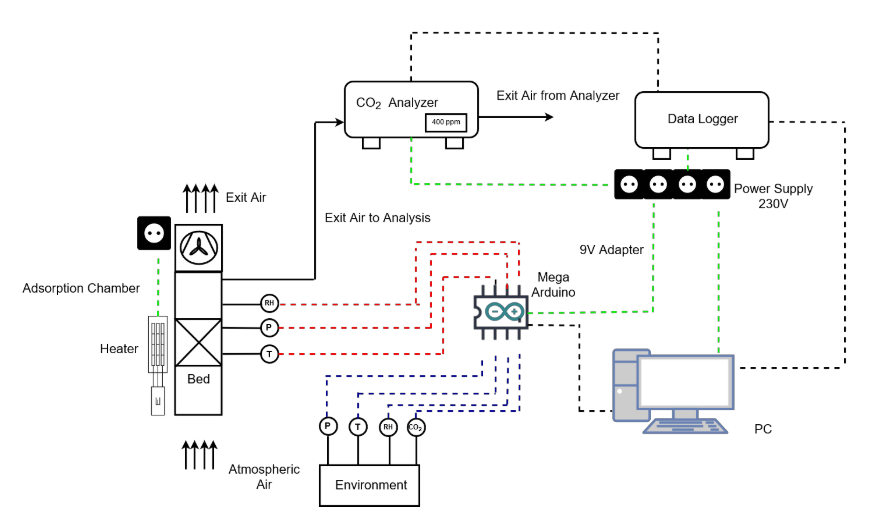
\includegraphics[width=\linewidth]{images/previouswork/zef1ads.png}
  \captionof{figure}{Schema of adsorption process \cite{Wagenaar2018}}
  \label{fig:zef1ads}
\end{minipage}%
\begin{minipage}{.5\textwidth}
  \centering
  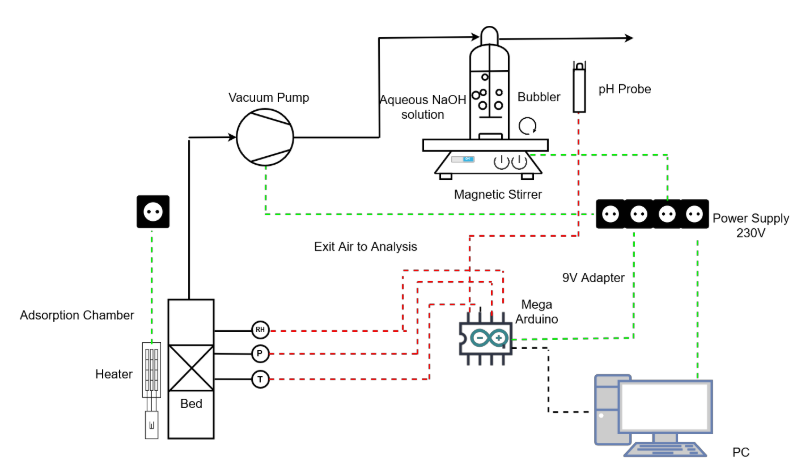
\includegraphics[width=\linewidth]{images/previouswork/zef1des.png}
  \captionof{figure}{Schema of desportion process \cite{Wagenaar2018}}
  \label{fig:zef1des}
\end{minipage}
\end{figure}

\begin{figure}[H]
    \centering
    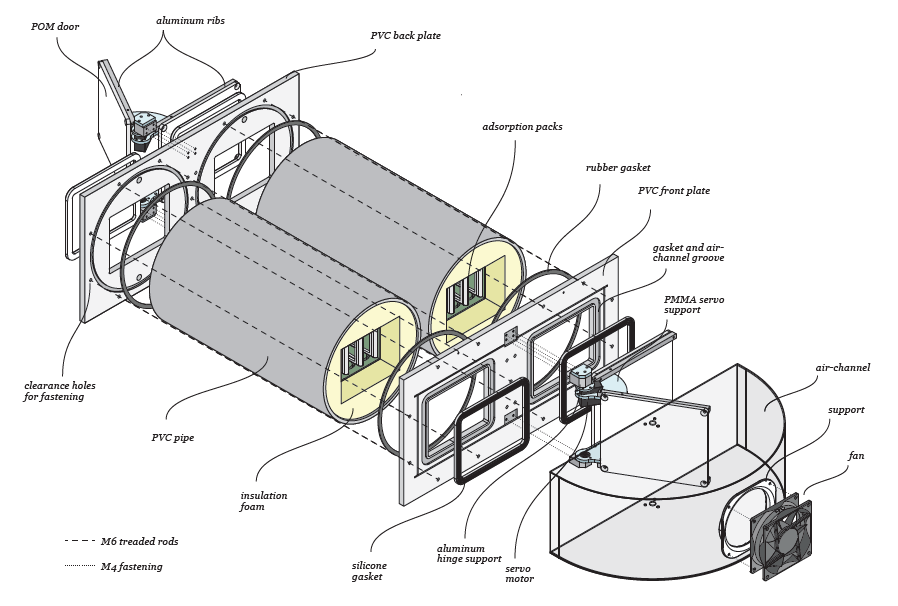
\includegraphics[width=\linewidth]{images/previouswork/zef1ass.png}
    \caption{Isometric view of the DAC unit assembly \cite{Azzalini2018}}
    \label{fig:zef1ass}
\end{figure}

\subsubsection{Further work}
The DAC team of ZEF 1 got a DAC system running from scratch. However, the heating and cooling systems were not installed. Hence, no system testing could be performed. Some of the relevant conclusions and recommendations put forward by the team was :

\begin{itemize}
    \item In order to address the fluctuations in sensor readings. Powering the sensors using a stable and constant 9V power adapter is required. 
    \item Selection of a cheaper sorbent material such as amine grafter sugarcane bagasse. 
    \item Since PEI is a non - newtonian fluid, higher $CO_2$ absorption might be observed in order to optimize the parameter. 
    \item Innovative designs might help in better heat utilization for the other sub-systems and can aid in the adsorption of $CO_2$ in DAC. 
    \item Testing with the heating and condensation units must be carried out. 
\end{itemize}

\subsection{ZEF II - the shift to monoliths}

During the time of ZEF II, the DAC system was still in a design phase and it was suggested by R. Berg to shift to monoliths in his MSc thesis report. His goal was to come up with a DAC system design that can be mass produced at a reasonable price. At this stage, ZEF still considered that batch process is the best way to approach DAC system as well. The reasons why he suggested this DAC system are \cite{Berg2018}: 
\begin{enumerate}
    \item Small size - can be mass produced easiliy and makes handling easier 
    \item Heat integration - allows heating using Peltier elements
    \item Functionality
    \item Exchangeable monolith
    \item Stand alone DAC - easily integrated with other systems. 
    \item Capture - captures $CO_2$ and water vapor. 
    \item Lower capture costs - R. Berg estimates $CO_2$ capture costs to about 123 euros per ton $CO_2$
\end{enumerate}

There were also students who had to study the $CO_2$ loading characteristics in PEI 10K and 1.2K to find the best candidate that could work best in the DAC system by studying the amount of $CO_2$ absorbed in the PEI. It was found that 10K PEI has slower kinetics than 1.2K PEI but absorbs less water compared to 1.2K. It was also found that active carbon is highly insulating and heating is slow. Thereby we have large heat demand for the desorbtion system which is very undesirable \cite{Laake2018}. This is where the shift from batch processing to continuous DAC system happened for ZEF. 


\subsection{ZEF III - continuous DAC system studies}

In order to study the feasibility of a continuous DAC system, the interns of ZEF III conducted various test farms to let PEI flow through and observations were made of the flow of PEI through the channels that were 3D printed. According to M. Sinha, these are the following observations made during the testing phase \cite{Sinha2018} : 

\subsubsection{Absorption}

\begin{enumerate}
    \item As the PEI layer goes down, the PEI stays more time on the plate and can absorb more $CO_2$ per kg of amine. A layer thickness of about 0.1 mm was recommended. 
    \item Direction of airflow has no effect on the amount of $CO_2$ absorbed by the sorbent. 
    \item Paper as a flow surface is found to have the lowest layer thickness, which is desired as elaborated in the first point. 
    \item Pre-wetting the flow surface is very essential to achieve a very good flow
    \item A honey comb structure must be used at the entry of the sorbent inorder to reduce surface tension effects. 
\end{enumerate}

\subsubsection{Desportion}

\begin{enumerate}
    \item Reaction of PEI and TEPA with metals s
    \item PEI600 and PEI1200 burning at 145 \degree C. 
    \item Proper enclosure must be ensured inorder to remove water vapor from the system. 
    \item Within 6 minutes, 80\% of the absorbed $CO_2$ could be desorbed in the desorption chamber. 
\end{enumerate}

Some of the recommendations given by M. Sinha were to study more on the flow of air as well and the difference a laminar or turbulent flow can make with $CO_2$ absorption. Study on the viscosity changes were also recommended to understand the flow of PEI better. Life cycle and mass transfer kinetics during the desorbtion process was also recommended.   



\subsection{ZEF IV - absorption \& desorbtion using PEI and TEPA}
\label{sec:zef4}

Given with the lack of literature and research on the amines PEI and TEPA. It was iminent that ZEF B.V had to find the data by themselves. Hence, previous Energy, Process and Technology students Bart Ovaa and Nuria Serrano Barthe were tasked study the events of PEI and TEPA under various loaded conditions of $H_{2}O$ and $CO_2$ in desporbtion \cite{Ovaa2019} and absorption \cite{NuriaSerranoBarthe2019} respectively for their MSc thesis. During this time, the designs for DAC V1.1 system was also made during with various design iterations and channel flow testing with physical conditions. To see where the maximum amount of $CO_2$ capture and easy desorbtion occurs. In order to summarize their findings : 

\begin{table}[H]
    \centering
    \begin{tabular}{|p{\linewidth/2}|p{\linewidth/2}|}
    \hline
        Absorbtion \cite{NuriaSerranoBarthe2019}  &  Desorbtion  \cite{Ovaa2019} \\
         \hline
         \hline
        Pure TEPA captures most $CO_2$ than pure PEI    &  $CO_2$ and $H_{2}O$ undergo physical adsorption initially. $CO_2$ later reacts to form carbamate. The inverse occurs during desorbtion  \\
        \hline
        High moisture content improves $CO_2$ loading in TEPA, opposite occurs in PEI   &    T and P are very important parameters and can determine the desorbtion capacity of the polyamine  \\
        \hline
        $CO_2$ capture occurs due to carbamate formation and higher desorption energy needed for making bicarbonates    &  Energy demand for desorbtion stems mainly from sensible heating the polyamine \\
        \hline
        
        
    \end{tabular}
    \caption{ZEF IV key findings \cite{NuriaSerranoBarthe2019} \cite{Ovaa2019}}
    \label{tab:ZEF4find}
\end{table}


In Table \ref{tab:ZEF4find}, we can find a summary of the thesis finding. However, it is best advised to read them before reading this report as they form the basis in which the current DAC system has been designed and the assumptions have been taken accordingly. 
















